\documentclass{standalone}
\usepackage{tikz}
\usetikzlibrary{patterns, positioning}
\usepackage[sfdefault]{ClearSans} %% option 'sfdefault' activates Clear Sans as the default text font
\usepackage[T1]{fontenc}

\begin{document}
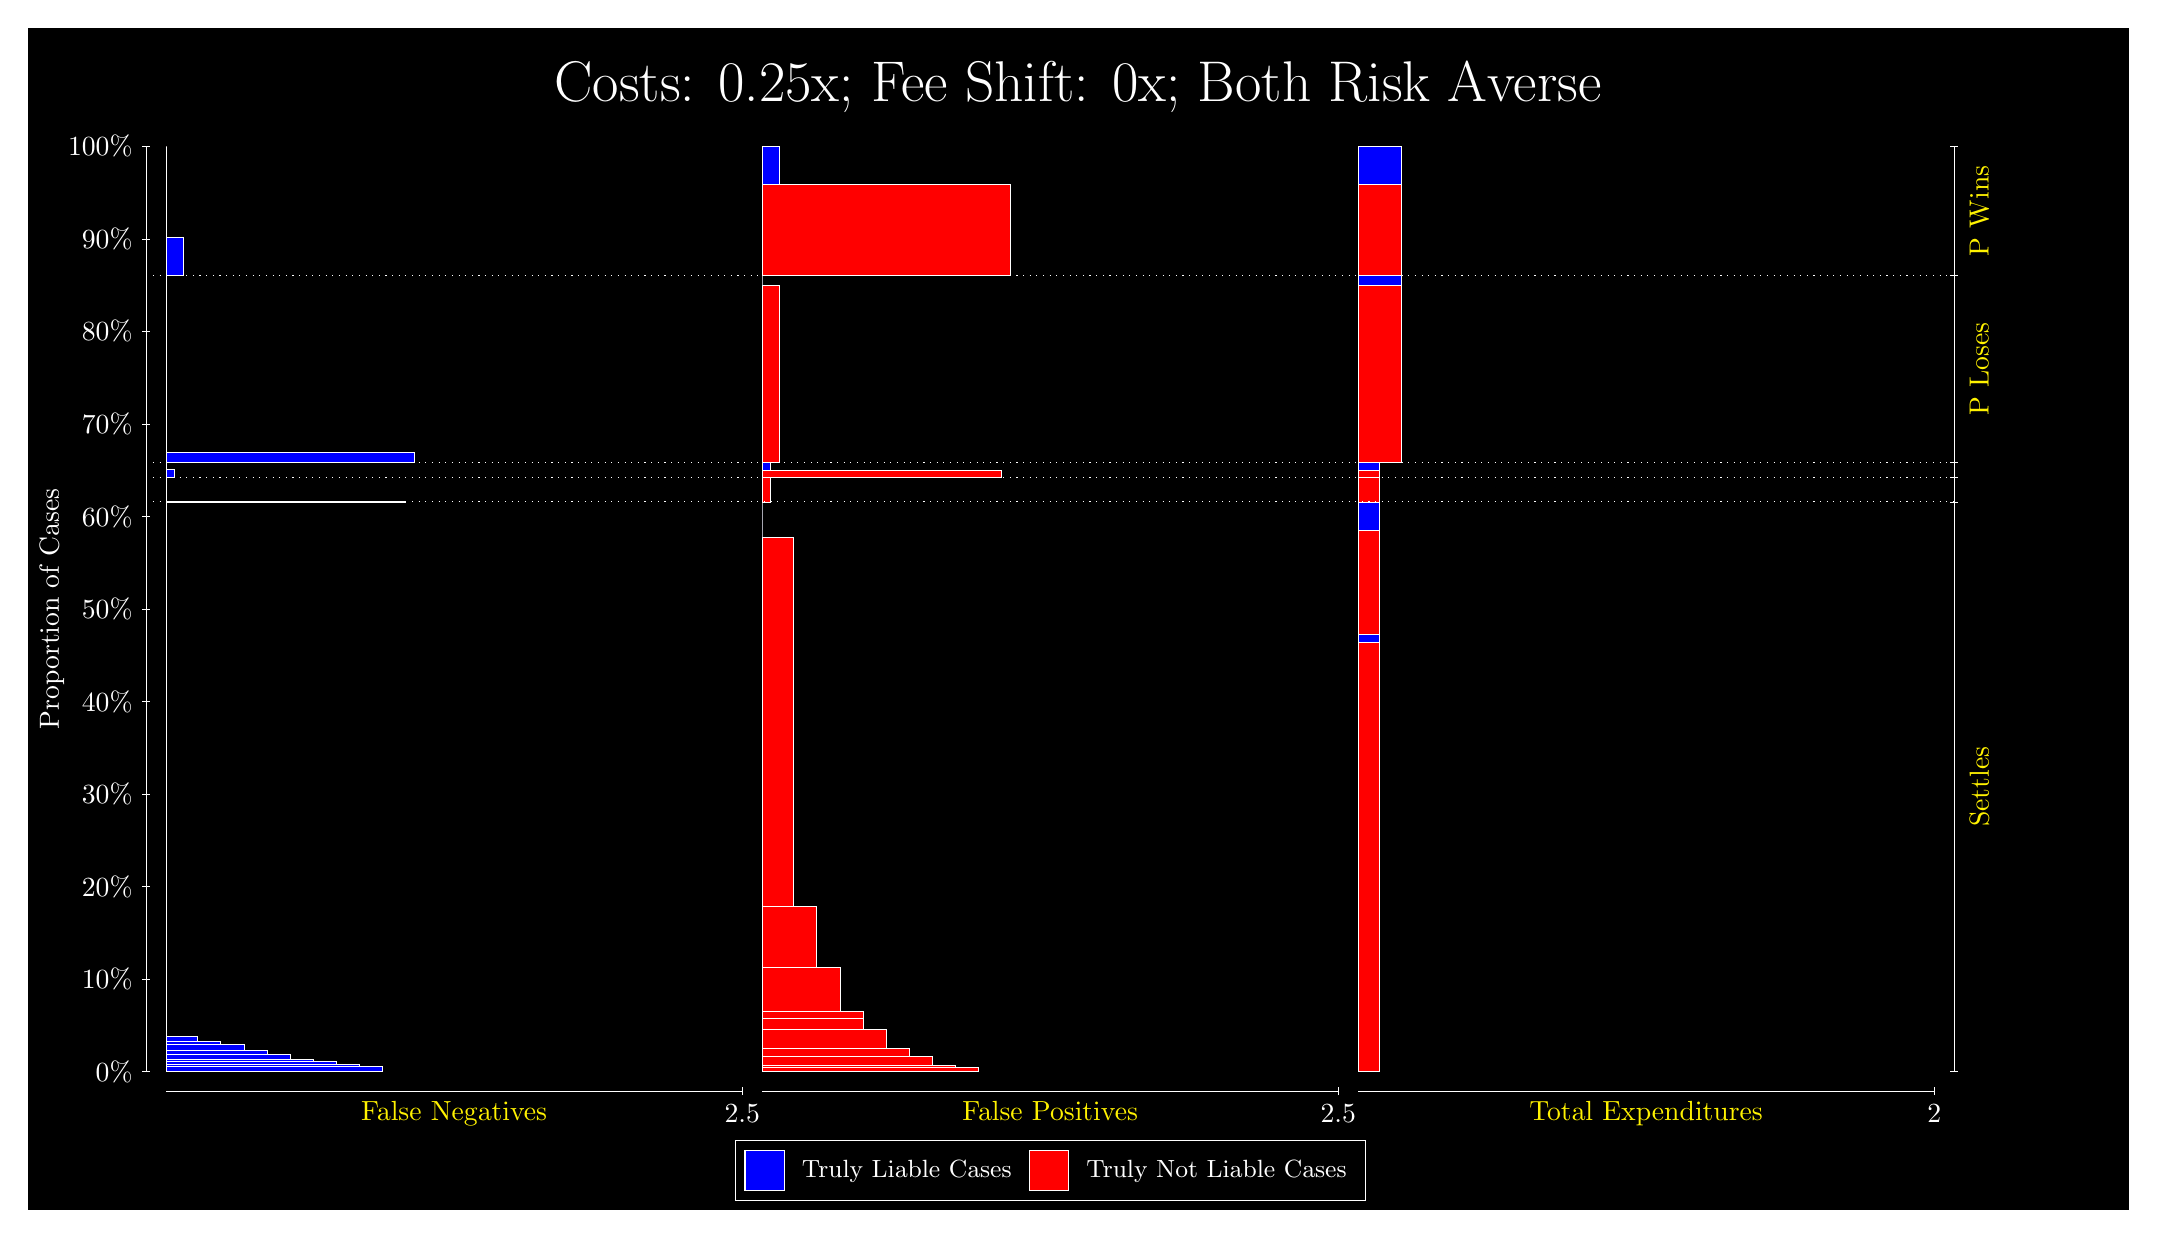
\begin{tikzpicture}
\draw[fill=black] (0,0) rectangle (26.667,15);
\draw[text=white] (0,13.5) rectangle (26.667,15) node[midway] {\huge Costs: 0.25x; Fee Shift: 0x; Both Risk Averse};
\draw[white, very thin] (1.5,1.75) -- (1.5,13.5);
\node[rotate=90, text=white, anchor=center] at (0.3, 7.625) {Proportion of Cases};
\draw[white, very thin] (1.45,1.75) -- (1.55,1.75);
\node[text=white, anchor=east] at (1.45, 1.75) {0\%};
\draw[white, very thin] (1.45,2.925) -- (1.55,2.925);
\node[text=white, anchor=east] at (1.45, 2.925) {10\%};
\draw[white, very thin] (1.45,4.1) -- (1.55,4.1);
\node[text=white, anchor=east] at (1.45, 4.1) {20\%};
\draw[white, very thin] (1.45,5.275) -- (1.55,5.275);
\node[text=white, anchor=east] at (1.45, 5.275) {30\%};
\draw[white, very thin] (1.45,6.45) -- (1.55,6.45);
\node[text=white, anchor=east] at (1.45, 6.45) {40\%};
\draw[white, very thin] (1.45,7.625) -- (1.55,7.625);
\node[text=white, anchor=east] at (1.45, 7.625) {50\%};
\draw[white, very thin] (1.45,8.8) -- (1.55,8.8);
\node[text=white, anchor=east] at (1.45, 8.8) {60\%};
\draw[white, very thin] (1.45,9.975) -- (1.55,9.975);
\node[text=white, anchor=east] at (1.45, 9.975) {70\%};
\draw[white, very thin] (1.45,11.15) -- (1.55,11.15);
\node[text=white, anchor=east] at (1.45, 11.15) {80\%};
\draw[white, very thin] (1.45,12.325) -- (1.55,12.325);
\node[text=white, anchor=east] at (1.45, 12.325) {90\%};
\draw[white, very thin] (1.45,13.5) -- (1.55,13.5);
\node[text=white, anchor=east] at (1.45, 13.5) {100\%};

\draw[white, very thin] (24.457,1.75) -- (24.457,13.5);
\draw[white, very thin] (24.407,1.75) -- (24.507,1.75);
\node[anchor=west] at (24.407, 1.75) {};
\draw[white, very thin] (24.407,8.984) -- (24.507,8.984);
\node[anchor=west] at (24.407, 8.984) {};
\draw[white, very thin] (24.407,9.2996) -- (24.507,9.2996);
\node[anchor=west] at (24.407, 9.2996) {};
\draw[white, very thin] (24.407,9.4854) -- (24.507,9.4854);
\node[anchor=west] at (24.407, 9.4854) {};
\draw[white, very thin] (24.407,11.86) -- (24.507,11.86);
\node[anchor=west] at (24.407, 11.86) {};
\draw[white, very thin] (24.407,13.5) -- (24.507,13.5);
\node[anchor=west] at (24.407, 13.5) {};

\draw[white, very thin, fill=blue] (1.75,1.75) rectangle (4.4946,1.8223);
\draw[white, very thin, fill=blue] (1.75,1.8223) rectangle (4.2018,1.8431);
\draw[white, very thin, fill=blue] (1.75,1.8431) rectangle (3.9091,1.8781);
\draw[white, very thin, fill=blue] (1.75,1.8781) rectangle (3.6163,1.9087);
\draw[white, very thin, fill=blue] (1.75,1.9087) rectangle (3.3236,1.973);
\draw[white, very thin, fill=blue] (1.75,1.973) rectangle (3.0308,2.0159);
\draw[white, very thin, fill=blue] (1.75,2.0159) rectangle (2.738,2.0981);
\draw[white, very thin, fill=blue] (1.75,2.0981) rectangle (2.4453,2.1348);
\draw[white, very thin, fill=blue] (1.75,2.1348) rectangle (2.1525,2.2012);
\draw[white, very thin, fill=red] (1.75,2.2012) rectangle (1.75,8.984);
\draw[white, very thin, fill=blue] (1.75,8.984) rectangle (4.7873,8.9921);
\draw[white, very thin, fill=red] (1.75,8.9921) rectangle (1.75,9.2996);
\draw[white, very thin, fill=blue] (1.75,9.2996) rectangle (1.8598,9.4003);
\draw[white, very thin, fill=red] (1.75,9.4003) rectangle (1.75,9.4854);
\draw[white, very thin, fill=blue] (1.75,9.4854) rectangle (4.8971,9.6122);
\draw[white, very thin, fill=red] (1.75,9.6122) rectangle (1.75,11.86);
\draw[white, very thin, fill=blue] (1.75,11.86) rectangle (1.9696,12.348);
\draw[white, very thin, fill=red] (1.75,12.348) rectangle (1.75,13.5);
\draw[white, very thin, fill=red] (9.3189,1.75) rectangle (12.063,1.8006);
\draw[white, very thin, fill=red] (9.3189,1.8006) rectangle (11.771,1.834);
\draw[white, very thin, fill=red] (9.3189,1.834) rectangle (11.478,1.9494);
\draw[white, very thin, fill=red] (9.3189,1.9494) rectangle (11.185,2.0454);
\draw[white, very thin, fill=red] (9.3189,2.0454) rectangle (10.892,2.2812);
\draw[white, very thin, fill=red] (9.3189,2.2812) rectangle (10.6,2.4224);
\draw[white, very thin, fill=red] (9.3189,2.4224) rectangle (10.6,2.5203);
\draw[white, very thin, fill=red] (9.3189,2.5203) rectangle (10.307,3.075);
\draw[white, very thin, fill=red] (9.3189,3.075) rectangle (10.014,3.8436);
\draw[white, very thin, fill=red] (9.3189,3.8436) rectangle (9.7214,8.5328);
\draw[white, very thin, fill=blue] (9.3189,8.5328) rectangle (9.3189,8.984);
\draw[white, very thin, fill=red] (9.3189,8.984) rectangle (9.4287,9.2915);
\draw[white, very thin, fill=blue] (9.3189,9.2915) rectangle (9.3189,9.2996);
\draw[white, very thin, fill=red] (9.3189,9.2996) rectangle (12.356,9.3847);
\draw[white, very thin, fill=blue] (9.3189,9.3847) rectangle (9.4287,9.4854);
\draw[white, very thin, fill=red] (9.3189,9.4854) rectangle (9.5384,11.733);
\draw[white, very thin, fill=blue] (9.3189,11.733) rectangle (9.3189,11.86);
\draw[white, very thin, fill=red] (9.3189,11.86) rectangle (12.466,13.012);
\draw[white, very thin, fill=blue] (9.3189,13.012) rectangle (9.5384,13.5);
\draw[white, very thin, fill=red] (16.888,1.75) rectangle (17.162,7.2078);
\draw[white, very thin, fill=blue] (16.888,7.2078) rectangle (17.162,7.3009);
\draw[white, very thin, fill=red] (16.888,7.3009) rectangle (17.162,8.6259);
\draw[white, very thin, fill=blue] (16.888,8.6259) rectangle (17.162,8.984);
\draw[white, very thin, fill=red] (16.888,8.984) rectangle (17.162,9.2915);
\draw[white, very thin, fill=blue] (16.888,9.2915) rectangle (17.162,9.2996);
\draw[white, very thin, fill=red] (16.888,9.2996) rectangle (17.162,9.3847);
\draw[white, very thin, fill=blue] (16.888,9.3847) rectangle (17.162,9.4854);
\draw[white, very thin, fill=red] (16.888,9.4854) rectangle (17.437,11.733);
\draw[white, very thin, fill=blue] (16.888,11.733) rectangle (17.437,11.86);
\draw[white, very thin, fill=red] (16.888,11.86) rectangle (17.437,13.012);
\draw[white, very thin, fill=blue] (16.888,13.012) rectangle (17.437,13.5);
\draw[white, dotted] (1.5,8.984) -- (24.457,8.984);
\draw[white, dotted] (1.5,9.2996) -- (24.457,9.2996);
\draw[white, dotted] (1.5,9.4854) -- (24.457,9.4854);
\draw[white, dotted] (1.5,11.86) -- (24.457,11.86);
\draw[white, very thin] (1.75,1.5) -- (9.0689,1.5);
\node[text=yellow, anchor=north] at (5.4094, 1.5) {False Negatives};
\draw[white, very thin] (9.0689,1.45) -- (9.0689,1.55);
\node[text=white, anchor=north] at (9.0689, 1.45) {2.5};

\draw[white, very thin] (9.3189,1.5) -- (16.638,1.5);
\node[text=yellow, anchor=north] at (12.978, 1.5) {False Positives};
\draw[white, very thin] (16.638,1.45) -- (16.638,1.55);
\node[text=white, anchor=north] at (16.638, 1.45) {2.5};

\draw[white, very thin] (16.888,1.5) -- (24.207,1.5);
\node[text=yellow, anchor=north] at (20.547, 1.5) {Total Expenditures};
\draw[white, very thin] (24.207,1.45) -- (24.207,1.55);
\node[text=white, anchor=north] at (24.207, 1.45) {2};

\node[text=yellow, centered, rotate=90] at (24.777, 5.367) {Settles};


\node[text=yellow, centered, rotate=90] at (24.777, 10.672) {P Loses};
\node[text=yellow, centered, rotate=90] at (24.777, 12.68) {P Wins};

\draw (12.978300999999998,1.5) node[draw=none] (baseCoordinate) {};
\begin{scope}[align=center]
        \matrix[scale=0.5, draw=white, below=0.5cm of baseCoordinate, nodes={draw}, column sep=0.1cm]{
            \node[rectangle, draw, minimum width=0.5cm, minimum height=0.5cm, fill=blue] {}; &
            \node[draw=none, font=\small, text=white] (B) {Truly Liable Cases}; &
            \node[rectangle, draw, minimum width=0.5cm, minimum height=0.5cm, fill=red] {}; &
            \node[draw=none, font=\small, text=white] (B) {Truly Not Liable Cases}; \\
            };
\end{scope}

\end{tikzpicture}
\end{document}